% ----------------------------------------------------------------- %
%             The Speech Signal Processing Toolkit (SPTK)           %
%             developed by SPTK Working Group                       %
%             http://sp-tk.sourceforge.net/                         %
% ----------------------------------------------------------------- %
%                                                                   %
%  Copyright (c) 1984-2007  Tokyo Institute of Technology           %
%                           Interdisciplinary Graduate School of    %
%                           Science and Engineering                 %
%                                                                   %
%                1996-2017  Nagoya Institute of Technology          %
%                           Department of Computer Science          %
%                                                                   %
% All rights reserved.                                              %
%                                                                   %
% Redistribution and use in source and binary forms, with or        %
% without modification, are permitted provided that the following   %
% conditions are met:                                               %
%                                                                   %
% - Redistributions of source code must retain the above copyright  %
%   notice, this list of conditions and the following disclaimer.   %
% - Redistributions in binary form must reproduce the above         %
%   copyright notice, this list of conditions and the following     %
%   disclaimer in the documentation and/or other materials provided %
%   with the distribution.                                          %
% - Neither the name of the SPTK working group nor the names of its %
%   contributors may be used to endorse or promote products derived %
%   from this software without specific prior written permission.   %
%                                                                   %
% THIS SOFTWARE IS PROVIDED BY THE COPYRIGHT HOLDERS AND            %
% CONTRIBUTORS "AS IS" AND ANY EXPRESS OR IMPLIED WARRANTIES,       %
% INCLUDING, BUT NOT LIMITED TO, THE IMPLIED WARRANTIES OF          %
% MERCHANTABILITY AND FITNESS FOR A PARTICULAR PURPOSE ARE          %
% DISCLAIMED. IN NO EVENT SHALL THE COPYRIGHT OWNER OR CONTRIBUTORS %
% BE LIABLE FOR ANY DIRECT, INDIRECT, INCIDENTAL, SPECIAL,          %
% EXEMPLARY, OR CONSEQUENTIAL DAMAGES (INCLUDING, BUT NOT LIMITED   %
% TO, PROCUREMENT OF SUBSTITUTE GOODS OR SERVICES; LOSS OF USE,     %
% DATA, OR PROFITS; OR BUSINESS INTERRUPTION) HOWEVER CAUSED AND ON %
% ANY THEORY OF LIABILITY, WHETHER IN CONTRACT, STRICT LIABILITY,   %
% OR TORT (INCLUDING NEGLIGENCE OR OTHERWISE) ARISING IN ANY WAY    %
% OUT OF THE USE OF THIS SOFTWARE, EVEN IF ADVISED OF THE           %
% POSSIBILITY OF SUCH DAMAGE.                                       %
% ----------------------------------------------------------------- %
\hypertarget{bcp}{}
\name{bcp}{block copy}{data operation}

\begin{synopsis}
\item[bcp] [ --l $l$ ]  [ --L $L$ ]  [ --n $n$ ]  [ --N $N$ ]
           [ --s $s$ ]  [ --S $S$ ]  [ --e $e$ ]  [ --f $f$ ]
\item[\ ~~~~~~~] [ +{\em type} ] [ {\em infile} ] 
\end{synopsis}

\begin{qsection}{DESCRIPTION}
	{\em bcp} copies data blocks from {\em infile} (or standard input) 
	to standard output, 
	and reformats them according to the command line options given.

	If the input format is ASCII, 
	the basic input unit is a sequence of letters
	and the output block is partitioned with carriage returns.
\end{qsection}

\begin{figure}[h]
\begin{center}
\leavevmode
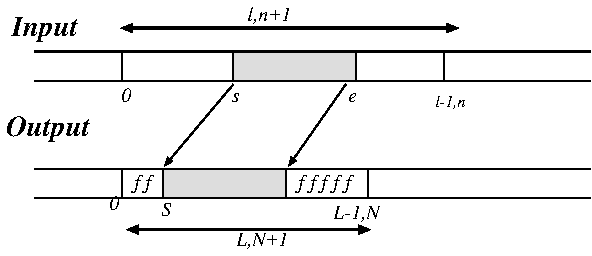
\includegraphics{fig/bcp.pdf}
\caption{Example of the bcp command}
\end{center}
\end{figure}

\begin{options}
	\argm{l}{l}{number of items contained 1 block}{512}
	\argm{L}{L}{number of destination block size}{N/A}
	\argm{n}{n}{order of items contained 1 block}{l-1}
	\argm{N}{N}{order of destination block size}{N/A}
	\argm{s}{s}{start number}{0}
	\argm{S}{S}{start number in destination block}{0}
	\argm{e}{e}{end number}{EOF}
	\argm{f}{f}{fill into empty block}{0}
	\argp{t}{data type\\ 
		\begin{tabular}{llcll} \\[-1ex]
         c & char (1 byte) & \quad &
         C & unsigned char (1 byte) \\
         s & short (2 bytes) & \quad &
                     S & unsigned short (2 bytes) \\
         i3 & int (3 bytes) & \quad &
                     I3 & unsigned int (3 bytes) \\
         i & int (4 bytes) & \quad &
                     I & unsigned int (4 bytes) \\
         l & long (4 bytes) & \quad &
                     L & unsigned long (4 bytes) \\
         le & long long (8 bytes) & \quad &
                     LE & unsigned long long (8 bytes) \\
         f & float (4 bytes) & \quad &
                     d & double (8 bytes) \\
			a & ASCII letter sequence\\
		\end{tabular}}{f}
\end{options}

\begin{qsection}{EXAMPLE}
Assume that {a(0), a(1), a(2), ... , a(20)}
 is contained in the input file {\em data.f}, written in float format.
If one wants to copy the array {a(1), a(2), ... , a(10)},
the following command can be used.
\begin{quote}
\verb!bcp +f -l 21 -s 1 -e 10 data.f > data.bcp!
\end{quote}

\par
A different example with respect to the same input file {\em data.f}
follows

\begin{quote}
\verb!bcp +f -l 21 -s 3 -e 5 -S 6 -L 10 data.f > data.bcp!
\end{quote}

In this example, the output block is
\begin{quote}
\verb!0, 0, 0, 0, 0, 0, a(3), a(4), a(5), 0!
\end{quote}
\end{qsection}

\begin{qsection}{NOTICE}
When both (--L and --N) or (--l and --n) are specified, latter argument is adopted.
\end{qsection}

\begin{qsection}{SEE ALSO}
\hyperlink{bcut}{bcut},
\hyperlink{merge}{merge},
\hyperlink{reverse}{reverse}
\end{qsection}
